\documentclass[13pt]{beamer}
\usepackage{graphicx}

\title{Obligatory Assignment 2 \\ Creating a Domain Specific Language using EMF}
\author{Tobias Birmili, Florian Hagenauer, Kacper Surdy}
\institute{University of Oslo}
\date{07.05.2012}

\usetheme{Darmstadt}
\usecolortheme{seahorse}

\setbeamercovered{transparent}

\begin{document}


\begin{frame}
	\titlepage
\end{frame}

\begin{frame}
	\frametitle{Creating the DSL Metamodel}
	\begin{itemize}
		\item Model Customer Journeys and Touchpoints
		\item Compare Customer Journeys to a reference
	\end{itemize}
	\begin{figure}[hbtp]
		\centering
		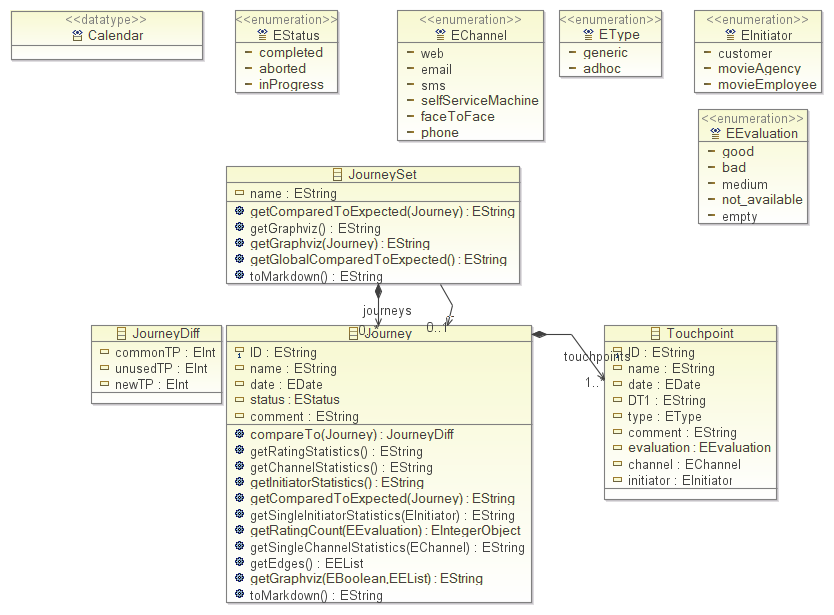
\includegraphics[scale=0.35]{img/JourneyModel.png}
	\end{figure}
\end{frame}

\begin{frame}
	\frametitle{Graphical Export}
	\begin{itemize}
		\item Generate Graphic to show the difference to the reference journey
		\item using GraphViz to generate SVG graphics
	\end{itemize}
	\only<1>{
		\begin{figure}[hbtp]
			\centering
			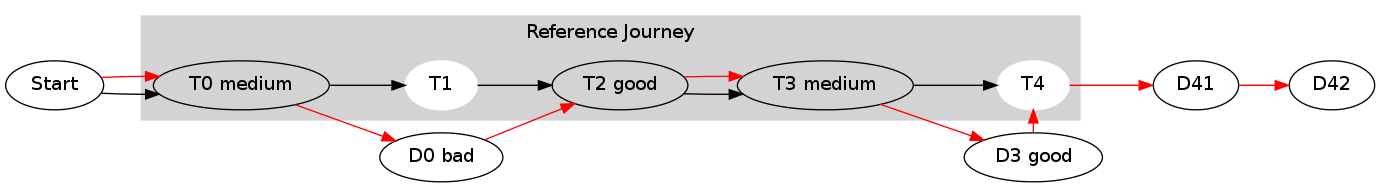
\includegraphics[scale=0.225]{img/sample_journey1.png}
		\end{figure}
	}
	\only<2>{
		\begin{figure}[hbtp]
			\centering
			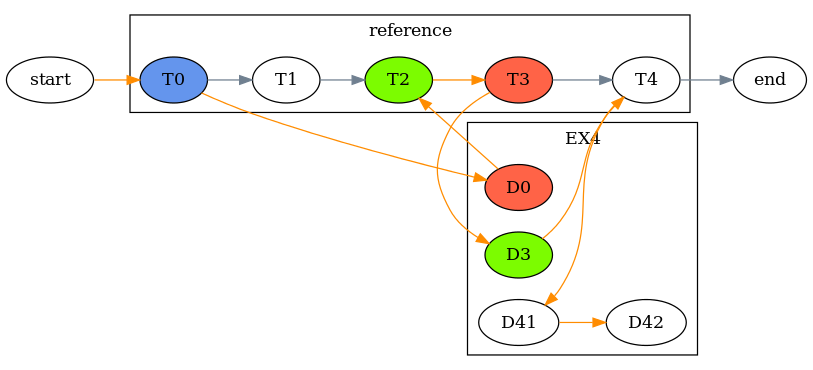
\includegraphics[scale=0.3]{img/sample_journey2.png}
		\end{figure}
	}
\end{frame}

\begin{frame}
	\frametitle{Merging Statistics and Export}
	\begin{itemize}
		\item Merge Statistics and Graphical Export into a HTML file
		\item Generate Markdown and Javascript Code
	\end{itemize}
	\begin{figure}[hbtp]
			\centering
			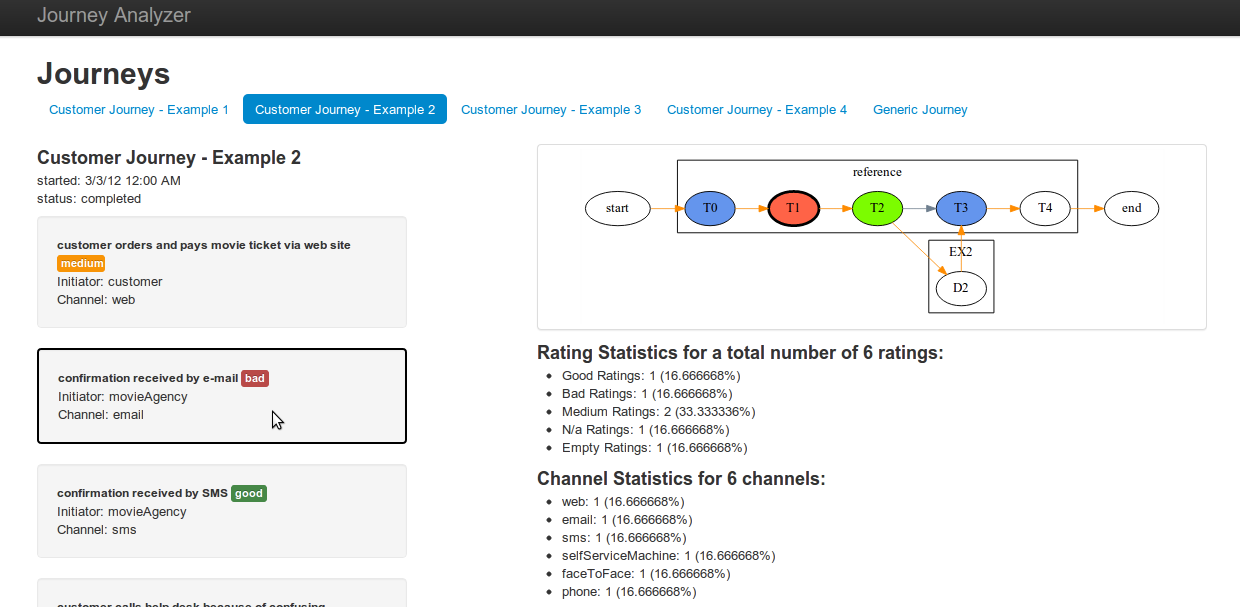
\includegraphics[scale=0.25]{img/merge_sample1.png}
	\end{figure}
\end{frame}	

\begin{frame}
	\frametitle{Livedemo - EMF \& Website}
	\begin{center} \huge{\textbf{LIVEDEMO}} \end{center}
\end{frame}

\end{document}